\chapter{Evaluation and Findings}



\section{Testing my implementation}
In order to keep tests fair, it is important to keep as much of the environment constant as possible between test iterations. Each iteration should have one variable that is changed so that the effects of this change can be easily observed and analysed. I have decied to investigate how changing the volume of traffic that is sent between client on a consumer network, effects the jitter with which the messages arrive.

The test is set up using the client hosted model where the clients are connected to the network on both an ethernet connection and WiFi. The host is connected to the router over ethernet cables that go through a switch. One client that will connect to the host is started on the same machine as the server; I will refer to this client as the ``localhost client''. Another client is connected directly to the router and I will refer to this one as ``ethernet client''. The last client that will connect to the host, is a laptop that is close to the router and connected over WiFi, this will be refered to as the ``WiFi client''.

Once the connection has been established, the server tickrate can be configured. This will be the variable that I will change and observe the effects of at each stage of the experiment. To minimise any external factors that could effect this experiment, I have also ran all tests at night when the network is under least stress.

\subsection{Capturing and analysing the results}
When writing my library, one of the most important features that I made sure to finish first is a custom wrapper for a logging library that would go on to be used extensively during the developement and testing. The code is written in such a way that any action that is done is logged under different logging levels depending on the nature of the information. One piece of information that is logged whenever a message is received by a client, is the time that has elapsed since the last message that has been received. This information can then in turn be used to calculate the jitter of incomming messages and this is what I have done in my experiment.

I have used a simple script that used regex expressions on each log file (one for each client and therefore three for each test), that would look for lines where the jitter information is logged and extract the number from the rest of the line. The result would be a file with 1 number per line which can then be fed into another program to generate graphs. The analysis of this data and some examples of the graphs produced in this way, can be found under section \ref{sec:jitter_results}.

In order to compare how varied the numbers were from one another, I have ran my results from each of the log files through a math function calculating the variance ($\sigma^2$) of the data. The analysis of this can be found in the section \ref{sec:variance_results}.

\newpage
\subsection{Jitter between WiFi and Ethernet connections} \label{sec:jitter_results}
My expectation for the results from this test, were that more anomolous values would be present in WiFi packets rather than Ethernet packets due to the higher chance of packet loss and less reliable connection technology. The jitter in WiFi data is also expected to be more varied than a wired connection.
After harvesting and extracting the data from my experiment, I have ended up with over 5000 numbers for each client and each test. Each number represents the time between two received messages arriving and so it is understandable that if a given packet takes longer then average to reach the client, a larger number will be produced however as a result when the next packet is received (after traveling for what can be assumed to be an average time), it is likely that the next value will be smaller than average. This nature, produces the zig-zag like shape that can be seen in the graphs where if there is a large spike in one direction, it is likely that the next data value, will then produce a large spike in the other direction. The graphs representing this data can be seen in figures \ref{fig:250ms_graph}, \ref{fig:64ms_graph} and \ref{fig:8ms_graph}. These graphs show the data for the WiFi client and the Ethernet client for 250ms, 64ms and 8ms server tick-rates respectively and each one has been limited to use the same amount of data to make the horisontal axis scale consistant. More graphs of this data, including data for different tickrates, can be found in the appendix.

For each dataset, the data turned out to be very similar; it can be seen that in general the data for the Ethernet client, arrived within 1 millisecond, however as expected, the data for the WiFi client appeared to be slightly more varied with most of the data arriving within 2 milliseconds of the average. Another anomaly that can be seen with the WiFi connection throughout each test, is that it is much more common for a ``random'' spike to occur. These spikes could occur due to several reasons. One example is that packet loss occured causing the wait for the next packet to essentially double. This can be seen in several instances through one value having an abnormally large value but not followed by an abnormally small value directly after.

An effect that can be observed with the different tick-rates, is that it is much less common for abnormally large or small, anomalous data to be seen in WiFi connections as the tick-rate gets faster. As the tick-rate increases, each anomalous result (whether it is due to packet loss or suboptimal routing) is much less impactful if there is another packet arriving soon after. An exception to this rule however can be seen in the 8ms test. The packets in the data for the 8ms test appear much more varied in general more anomalous spikes can be seen in both WiFi and Ethernet data (despite this trend being more obvious in WiFi data). To show these anomalous spikes, I have made the scale 2.5ms per horisontal line instead of 1ms like it is on the other graphs. Unfortunately, it is unclear why this exception occurs in this test when in every other test, the varience can be seen to be getting smaller.

\newpage
\begin{figure}[p]
  \centering
  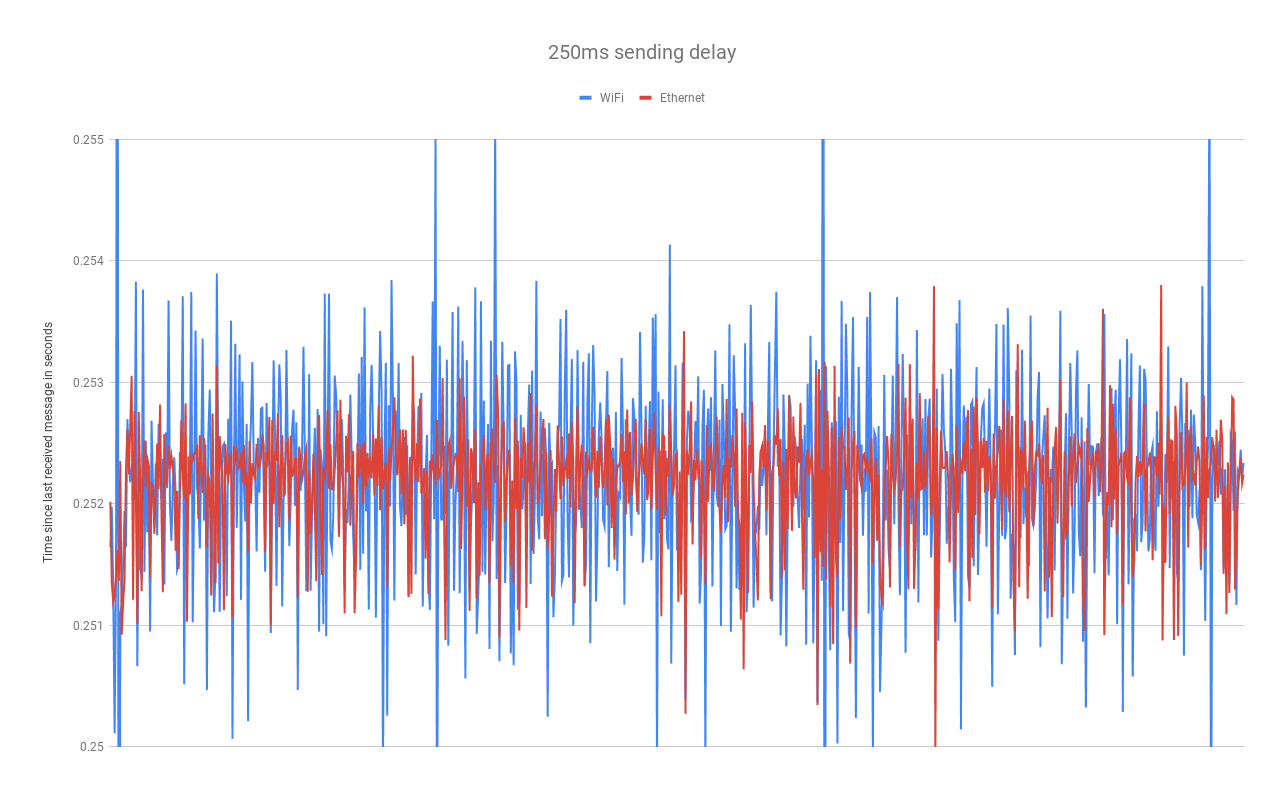
\includegraphics[width=\textwidth]{Graphs/250ms_delay}
  \caption{250ms Delay}
  \label{fig:250ms_graph}
\end{figure}

\begin{figure}[p]
  \centering
  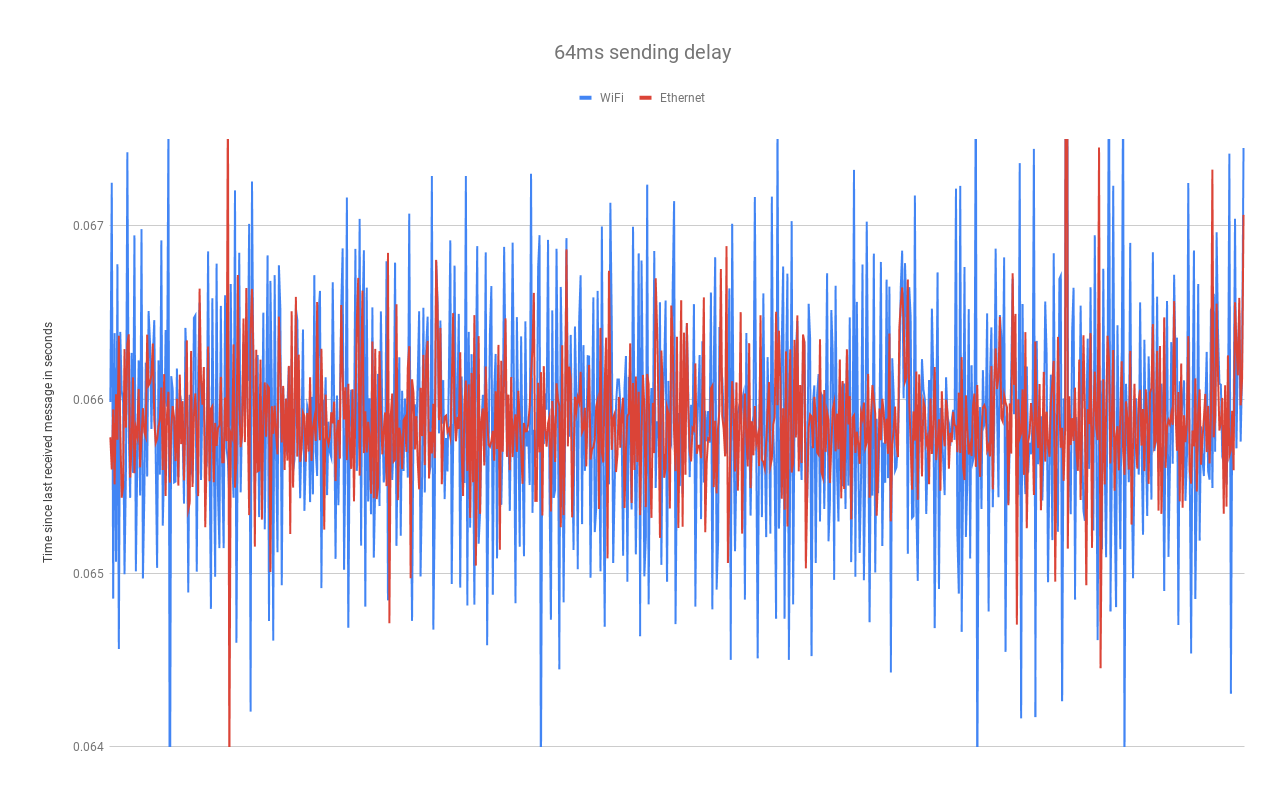
\includegraphics[width=\textwidth]{Graphs/64ms_delay}
  \caption{64ms Delay}
  \label{fig:64ms_graph}
\end{figure}

\begin{figure}[p]
  \centering
  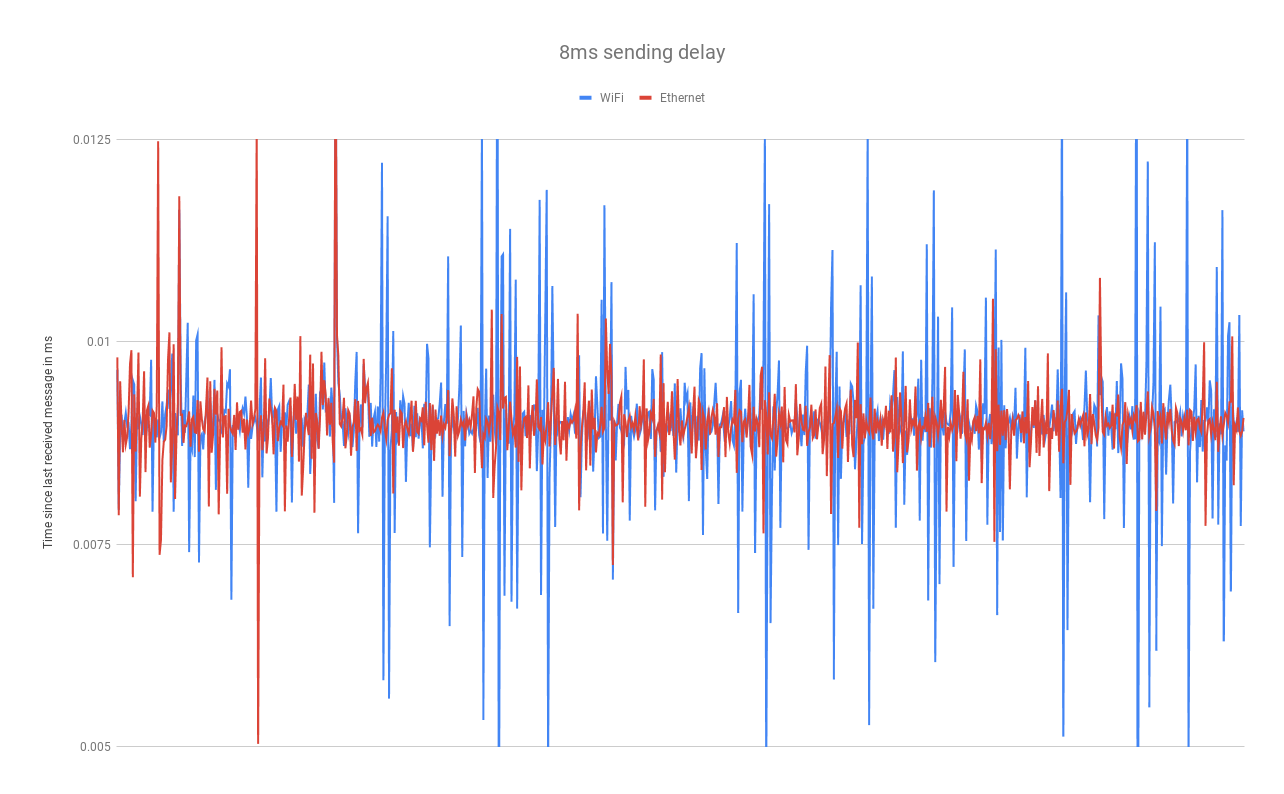
\includegraphics[width=\textwidth]{Graphs/8ms_delay}
  \caption{8ms Delay}
  \label{fig:8ms_graph}
\end{figure}



\subsection{Calculating the variance in jitter}\label{sec:variance_results}
The next question that I was interested in anwsering was: Objectively, which collection of gathered data, had the least variance in it? This data can be seen represented in a bar chart in figure \ref{fig:jitter_variance}. I have found that the $\sigma^2$ values for WiFi at the tickrate of 500 and 1000 milliseconds, were much larger than the other results due to having to wait for a much longer time if a packet was lost. Even when not considering these anomalous values however, it can be seen that the varience in the receiving rate is on average 30\% larger than the average of ethernet and localhost data.

 even the localhost client experianced a certain level of jitter. This is likely be due to the operating system prioritising certain programs over others as well how the NIC hardware and winsock manages sending and receiving of data.

Another surprising result was once again seen at the 8ms test. Following on from the previous section, it can be seen that he variance of the data incereases when compared to the other results despite what would intuitively be the most ``reliable'' constant stream of data. The fact that the rise can be seen in all three clients, indicates that there may be some external factor (such as my computer's NIC or consumer grade router hardware), that interferes with these results. In general, it is unlikely to see broadcast rates higher than 63Hz (around 16ms delay).

\begin{figure}[p]
  \centering
  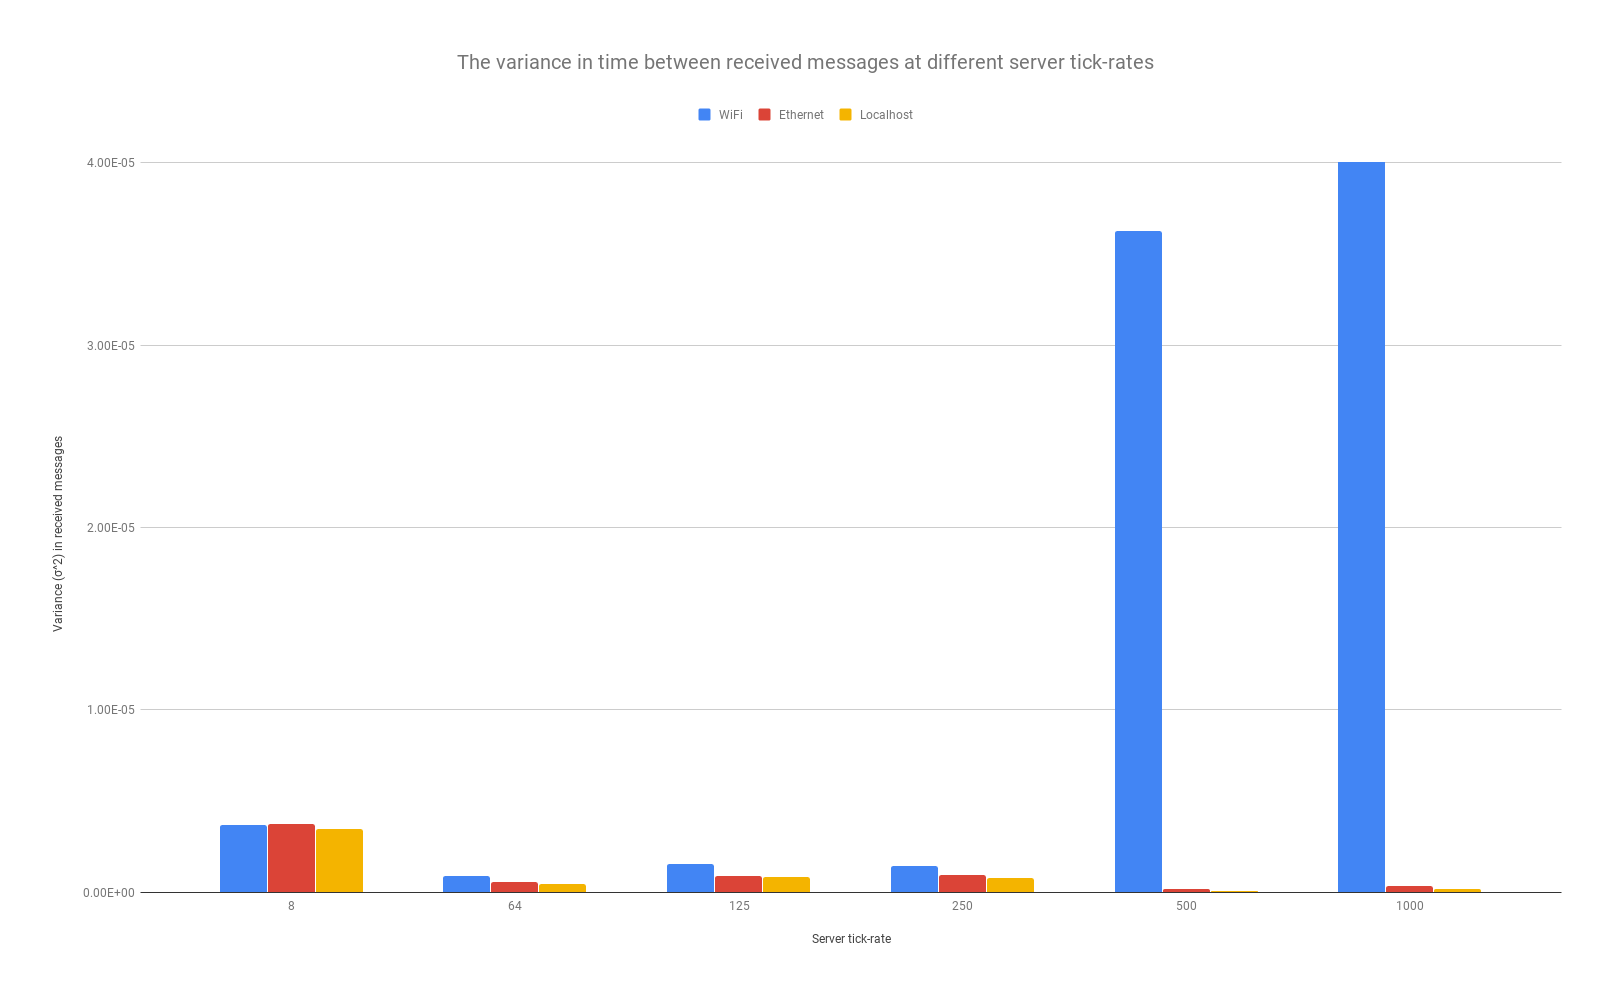
\includegraphics[width=\textwidth]{Graphs/jitter_variance}
  \caption{Graph showing the variance in the delay between receiving messages.}
  \label{fig:jitter_variance}
\end{figure}


\chapter{Conclusion}
